\documentclass[a4paper]{article}

\usepackage[margin=1in]{geometry} 
\usepackage{amsmath,amsthm,amssymb}
\usepackage{float}
\usepackage{graphicx}
\usepackage[dvipsnames]{xcolor}
\usepackage[UKenglish]{isodate}
\origdate
\cleanlookdateon
\usepackage[hidelinks]{hyperref}
\urlstyle{same}
\usepackage{tocloft}
\renewcommand{\cftsecleader}{\cftdotfill{\cftdotsep}}
\renewcommand{\baselinestretch}{1.25} 
\usepackage{enumitem}
\usepackage{framed}
\usepackage[T1]{fontenc}
\usepackage{kpfonts}
\usepackage{csquotes}
\usepackage{listings}
\usepackage[scaled]{beramono}
\usepackage{lscape}
\usepackage{multirow}
\usepackage{makecell}
\usepackage{graphbox}
\usepackage{pythonhighlight}

\definecolor{eclipseStrings}{RGB}{42,0.0,255}
\definecolor{eclipseKeywords}{RGB}{127,0,85}
\colorlet{numb}{magenta!60!black}

\lstdefinelanguage{json}{
    basicstyle=\normalfont\ttfamily,
    commentstyle=\color{eclipseStrings}, % style of comment
    stringstyle=\color{eclipseKeywords}, % style of strings
    numbers=left,
    numberstyle=\scriptsize,
    stepnumber=1,
    numbersep=8pt,
    showstringspaces=false,
    breaklines=true,
    frame=lines,
    backgroundcolor=\color{white},
    string=[s]{"}{"},
    comment=[l]{:\ "},
    morecomment=[l]{:"},
    literate=
        *{0}{{{\color{numb}0}}}{1}
         {1}{{{\color{numb}1}}}{1}
         {2}{{{\color{numb}2}}}{1}
         {3}{{{\color{numb}3}}}{1}
         {4}{{{\color{numb}4}}}{1}
         {5}{{{\color{numb}5}}}{1}
         {6}{{{\color{numb}6}}}{1}
         {7}{{{\color{numb}7}}}{1}
         {8}{{{\color{numb}8}}}{1}
         {9}{{{\color{numb}9}}}{1}
}


\begin{document}
\title{Finals Summary\\[0.1cm]
    \large 50.012 Networks, Elective 2019}
\author{Tey Siew Wen}
\date{06 Feb 2020}

\maketitle

\begin{table}[H]
    \centering
    \begin{tabular}{|l|l|}
    \hline
    \multicolumn{1}{|c|}{\textbf{Topic}} & \multicolumn{1}{c|}{\textbf{Specific Sections}}                                                                                                                  \\ \hline
    TCP Congestion Error                 & \begin{tabular}[c]{@{}l@{}}Lecture 10: Congestion Control,\\ Lecture 11: TCP Wrapup\end{tabular}                                                                 \\ \hline
    Network Layer                        & \begin{tabular}[c]{@{}l@{}}Lecture 13: Network Layer Overview,\\ Lecture 14: IP Addressing,\\ Lecture 15: Routing Algorithms,\\ Lecture 16: Routing\end{tabular} \\ \hline
    Link Layer \& Synthesis              & Lecture 19: Link Layer                                                                                                                                           \\ \hline
    Wireless and Mobile Networks         & Lecture 21: Wireless Networks                                                                                                                                    \\ \hline
    \end{tabular}
\end{table}

\newpage
\section{Lecture 10: Congestion Control}
\subsection{Principles of Flow Control}
\begin{itemize}
    \item Receiver controls sender so the sender won't overflow receiver's buffer by transmitting too much/too fast
    \begin{itemize}[label=$\circ$]
        \item Application may remove data from TCP socket buffers
    \end{itemize}
    \item Receiver includes a \texttt{rwnd} (receiver window) value in TCP header of receiver-to-sender segments
    \begin{itemize}[label=$\circ$]
        \item \texttt{RcvBuffer}
    \end{itemize}
\end{itemize}

\subsection{Principles of Congestion Control}
\begin{itemize}
    \item Congestion Control $\neq$ Flow Control!
    \item Mainfestations
    \begin{itemize}[label=$\circ$]
        \item Buffer Overflow at Routers: Lost Packets
        \item Queueing in Router buffers: Long Delay
    \end{itemize}
\end{itemize}
\noindent When packets are lost, any upstream transmission capacity used for that packet is wasted.

\subsubsection{Scenario 1: One Router w/ Infinite Buffers}
\begin{itemize}
    \item Assuming no retransmission
\end{itemize}

\subsubsection{One Router w/ Finite Buffers}
Assumptions for idealized case
\begin{itemize}
    \item Sender knows when router buffers available
    \item Sender sends only when router buffers available
\end{itemize}
Transfer rates
\begin{itemize}
    \item $\lambda_{\text{in}} = \lambda_{\text{out}}$: Application-layer input = output
    \item $\lambda_{\text{in}}' \geq \lambda_{\text{in}}$: Transport-layer input includes retransmissions
\end{itemize}

\subsubsection{TCP Congestion Controls}
\noindent\textbf{Increase sender's transmission rate until loss occurs}
\begin{itemize}
    \item Additive Increase: Increase cwnd (congestion window) by 1 MSS every RTT until loss detected
    \item Multiplicate Increase: Reduce cwnd in half after loss
\end{itemize}

\newpage
\section{Lecture 11: TCP Wrapup}
\subsection{TCP Congestion Control}
A summary code for the sections discussed below:
\begin{python}
    cwnd = MSS
    while connected:
    if time < slow_start_duration:
        cwnd *= 2
        if receive_ACK: 
        cwnd += MSS
    else: # congestion-avoidance state
        if receive_ACK:
        cwnd += MSS*(MSS/cwnd)
\end{python}
\begin{figure}[H]
    \centering
    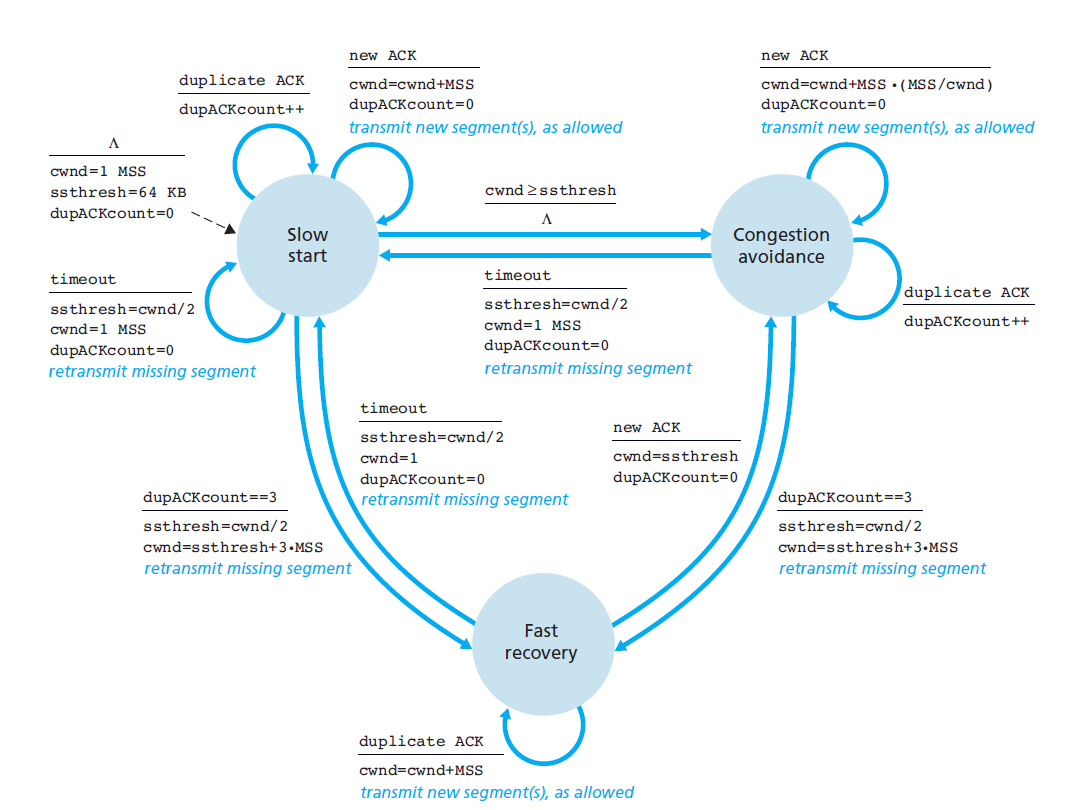
\includegraphics[width=0.9\linewidth, align=c]{images/TCPCongestionControl.PNG}
\end{figure}

\subsubsection{Start Connection: Slow Start}
When connection begins, increase rate exponentially until first loss event. (Initial rate is slow but ramps up very fast)
\begin{enumerate}
    \item Initial \texttt{cwnd}: 1 MSS (maximum segment size)
    \item Double \texttt{cwnd} every RTT
    \begin{itemize}
        \item It is doubled with the formula: $cwnd = cwnd + MSS * \displaystyle\frac{cwnd}{mss}$
    \end{itemize}
    \item Increment \texttt{cwnd} for every ACK received
\end{enumerate}

\subsubsection{Congestion-avoidance state}
Window grows exponentially in \textbf{slow start} to threshold, then grows linearly during the congestion-avoidance (CA) state. 
\begin{itemize}
    \item The inexponential increase is switched to linear when \texttt{cwnd} gets to half of its value before timeout.
    \item On loss event, \texttt{ssthresh}=0.5\texttt{*cwnd} before loss event.
\end{itemize}
In the CA state, the congestion window is increased by $\displaystyle\frac{1}{k}$.
\begin{itemize}
    \item where $k$ = $\displaystyle\frac{cwnd}{mss}$
\end{itemize}

\subsubsection{Explicit Congestion Notification (ECN)}
\paragraph{Network-assisted congestion control}
\begin{itemize}
    \item 2 bits in IP header (ToS field) marked by network router to indicate congestion
    \item Receiver sets ECE bit on ACK to notify sender of congestion
\end{itemize}

\subsubsection{Calculating TCP Throughput}
Ignoring slow start and assuming there is always data to send,
$$\text{TCP Throughput} = \frac{3}{4}*\frac{W}{RTT}$$
\begin{itemize}
    \item where $W$: window size in bytes where loss occurs
\end{itemize}
\begin{figure}[H]
    \centering
    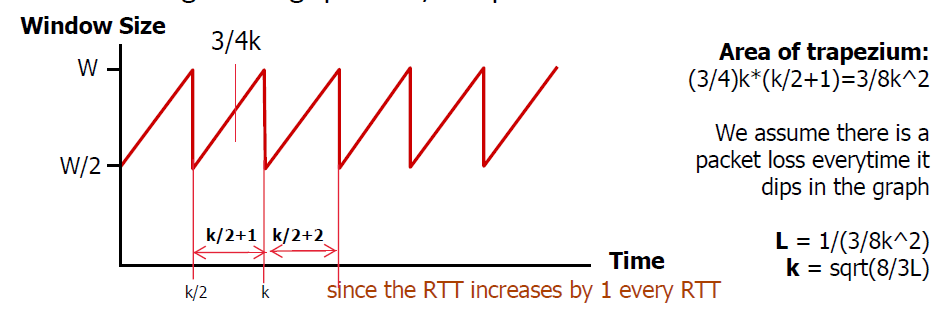
\includegraphics[width=0.7\linewidth, align=c]{images/tcp_throughput.PNG}
\end{figure}

\paragraph{Calculating Segment Loss Probability, L}\mbox{}\\
e.g. given 1500 byte segments, 100ms RTT, 10Gbps throughput, requires average 83,333 in-flight segments
\begin{align*}
    10^7 &=  \frac{1.22\times1500}{100\times10^{-3}*\sqrt{L}}\\
    L &= 2\times 10^{-10}
\end{align*}

\newpage
\subsubsection{TCP Fairness}
\begin{itemize}
    \item Goal: For $n$ TCP sessions sharing same bottleneck link of bandwidth $R$, each should have $\displaystyle\frac{R}{K}$ rate.
    \item Implementation via Additive Increase and Multiplicate Decrease
\end{itemize}
\begin{figure}[H]
    \centering
    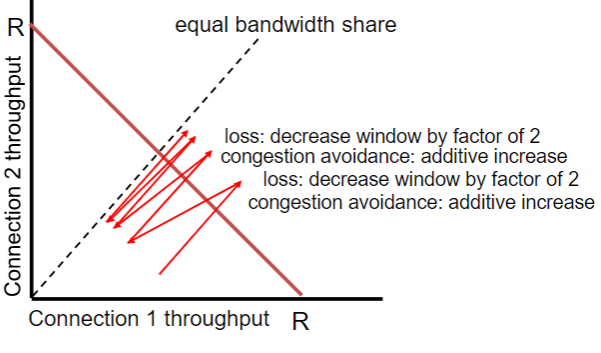
\includegraphics[width=0.7\linewidth, align=c]{images/tcp_fairness.PNG}
\end{figure}

\newpage
\section{Lecture 13: Network Layer Overview}
\subsection{Two Key Network-Layer Functions}
\begin{enumerate}
    \item \textit{Forwarding}: Router-local action of transferring a packet from an input link interface to the appropriate output link interface. (Data Plane)
    \item \textit{Routing}: Network-wide process that determines the end-to-end paths that packets take from source to destination. (Control Plane)
\end{enumerate}

\noindent\textbf{Control Plane Approaches:}
\begin{enumerate}
    \item Traditional Routing Algorithms: Implemented in Routers
    \begin{itemize}[label=$\circ$]
        \item Per-router control plane: Individual routing algorithm components in each and every router interact in the control plane
    \end{itemize}
    \item Software-defined Networking (SDN): Implemented in remote servers
    \begin{itemize}[label=$\circ$]
        \item A distinct controller interacts with local control agents
    \end{itemize}
\end{enumerate}

\noindent\textbf{Overview}
\begin{table}[H]
    \setcellgapes{5pt}
    \centering\makegapedcells
    \begin{tabular}{|l|l|}
    \hline
    \multicolumn{1}{|c|}{\textbf{Input port functions}} & \multicolumn{1}{c|}{\textbf{Output port functions}} \\ \hline
    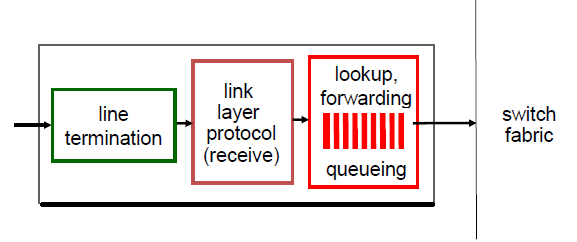
\includegraphics[width=0.45\linewidth, align=c]{images/input_port2.png} & 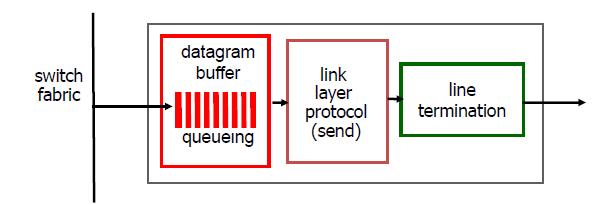
\includegraphics[width=0.45\linewidth, align=c]{images/output_port.png} \\ \hline
    \end{tabular}
\end{table}

\subsection{Input Processing}
Typical Forwarding Process:
\begin{figure}[H]
    \centering
    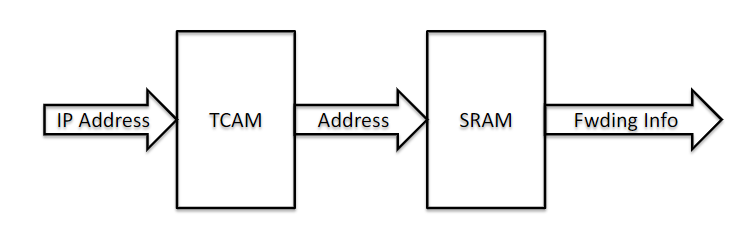
\includegraphics[width=0.7\linewidth, align=c]{images/forwarding_diagram.png}
\end{figure}
\begin{enumerate}
    \item Every router has a \textbf{forwarding table}, which is computed and updated by its routing processor, and \textbf{stored at the input port}.
    \begin{itemize}[label=$\circ$]
        \item A router forwards a packet by examining the value of a field in the arriving packet’s header, and then using this header value to index into the router’s forwarding table.
        \item The value stored in the forwarding table entry for that header indicates the router’s outgoing link interface to which that packet is to be forwarded.
        \item The value to be examined in the packet's header is determined by the \hyperref[routealgo]{\textcolor{blue}{routing algorithm}}.
    \end{itemize}
    \newpage
    \item The routing processor also stores a \textbf{shadow copy}, typically stored at each input port.
    \begin{itemize}[label=$\circ$]
        \item With a shadow copy, forwarding decisions can be made locally, at each input port, without invoking the centralized routing processor on a per-packet basis
        \item This helps to avoid a centralized processing bottleneck.
    \end{itemize}
    \item After determining the outgoing link interface, the packet is forwarded from the the router's input ports to its output ports via \textbf{switching fabrics}.
\end{enumerate}

\subsubsection{Switching Fabrics}
There are 3 types.
\begin{enumerate}
    \item Memory
    \begin{itemize}[label=$\circ$]
        \item An input port with an arriving packet first signaled the routing processor via an interrupt. The packet was then copied from the input port into processor memory.
        \item The routing processor then extract the destination addr from the header, looked up the appropriate output port in the forwarding table, and copied the packet to the output port’s buffers.
        \item If the memory bandwidth is such that B packets per second can be written into, or read from, memory, then the \textbf{overall forwarding throughput} (the total rate at which packets are transferred from input ports to output ports) \textbf{must be less than $\displaystyle\frac{B}{2}$}.
        \item Two packets cannot be forwarded at the same time, even if they have different destination ports, since only one memory read/write over the shared system bus can be done at a time.
    \end{itemize}
    \begin{figure}[H]
        \centering
        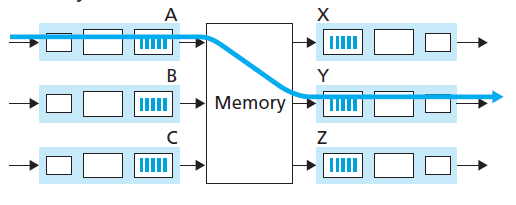
\includegraphics[width=0.5\linewidth, align=c]{images/switching_memory.png}
    \end{figure}
    \item Bus
    \begin{itemize}
        \item The packet is transferred directly from the input port to the output port over a shared bus, without intervention by the routing processor
        \item The input port pre-pend a switch-internal label (header) to the packet to indicate the local output port for the packet
        \item The packet is received by all output ports, but only the port that matches the label will keep the packet. The label is then removed at the output port.
        \item \textbf{Bus Contention}: Only one packet can board the bus at a time. Hence, the switching speed of the router is limited to the bus speed and transmitting the packet onto the bus 
    \end{itemize}
    \begin{figure}[H]
        \centering
        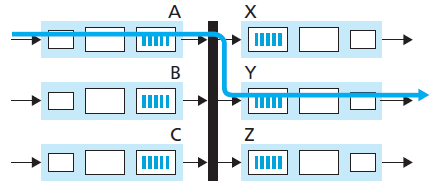
\includegraphics[width=0.5\linewidth, align=c]{images/switching_bus.png}
    \end{figure}
    \item Crossbar
    \begin{itemize}
        \item An interconnection network consisting of $2N$ buses that connect $N$ input ports to $N$ output ports
        \item There is a switch fabric controller to open/close cross points of the horizontal and vertical bus
        \item Capable of forwarding multiple packets in parallel.
        \item Initially developed to connect processors in multiprocessor.
    \end{itemize}
    \begin{figure}[H]
        \centering
        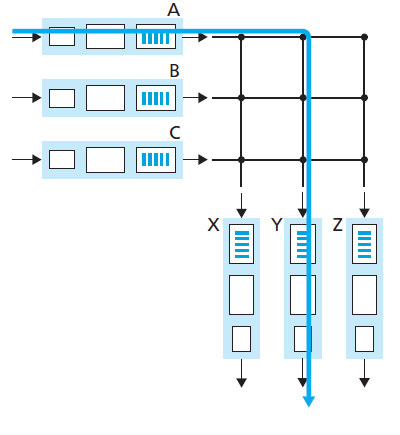
\includegraphics[width=0.5\linewidth, align=c]{images/switching_crossbar.png}
    \end{figure}
\end{enumerate}
\subsubsection{Input Port Queueing}
Since the switching fabric operates slower than the input ports, queueing at input queues may cause the input buffer to overflow. Packet loss will then occur when no memory is available to store arriving packets.

\bigskip
\noindent\textbf{Head of the Line (HOL) Blocking}

\bigskip
\noindent Queued datagram at front of queue prevents others in queue from moving forward
\begin{figure}[H]
    \centering
    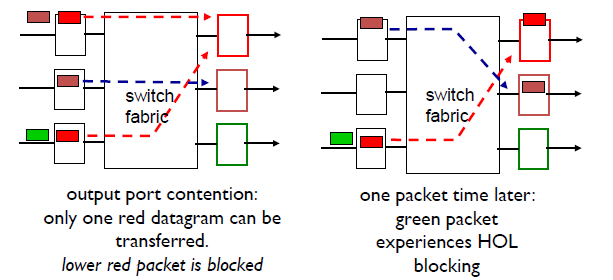
\includegraphics[width=0.5\linewidth, align=c]{images/hol_blocking.png}
\end{figure}

\subsubsection{Output Processing}
Output port processing takes packets that have been stored in the output port’s memory and transmits them over the output link. This includes selecting and de-queueing packets for transmission, and performing the needed linklayer and physical-layer transmission functions.

\bigskip

\noindent If the datagrams arrive from fabric faster than the transmission rate, buffering will be required. \textbf{Packet loss may occur} due to congestion and lack of buffers.
\subsection{Routing Algorithms}
\label{routealgo}
\begin{itemize}
    \item \textit{Destination-based forwarding}
    \begin{itemize}[label=$\circ$]
        \item Destination address range is the index for a particular link interface
        \item However there are times ranges don't divide up nicely
    \end{itemize}
    \item \textit{Longest Prefix Matching}
    \begin{itemize}[label=$\circ$]
        \item Longest address prefix is the index for matching destination addr
        \item Performed using Ternary Content Addressable Memories (TCAMs)
    \end{itemize}
\end{itemize}
e.g of longest prefix matching. given
\begin{table}[H]
    \centering
    \begin{tabular}{|l|l|}
    \hline
    \multicolumn{1}{|c|}{\textbf{Destination Address Range}} & \multicolumn{1}{c|}{\textbf{Link Interface}} \\ \hline
    1100 1000 0001 0111 0010*** **** ****                    & 0                                            \\ \hline
    1100 1000 0001 0111 0011*** **** ****                    & 1                                            \\ \hline
    1100 1000 0001 0111 0011000 **** ****                    & 2                                            \\ \hline
    otherwise                                                & 3                                            \\ \hline
    \end{tabular}
\end{table}
\begin{enumerate}[label=\alph*)]
    \item \textbf{1100 1000 00010111 0010}110 1011 0110: 0
    \item \textbf{1100 1000 00010111 0011000} 1011 0110: 2
    \item \textbf{1100 1000 00010111 0011}001 1011 0110: 1
\end{enumerate}

\subsubsection{Ternary Content-addressable memory (TCAMs)}
\begin{itemize}
    \item A specialized type of high-speed memory that searches its entire contents in a single clock cycle. 
    \begin{itemize}[label=$\circ$]
        \item More power, more area and higher latency than SRAM
        \item To retrieve data on RAM, the operating system (OS) must provide the memory address where the data is stored. 
        \item Data stored on CAM can be accessed by performing a query for the content itself, and the memory retrieves the addresses where that data can be found.
        \item Performs parallel processing 
    \end{itemize}
    \item Able to store and query data using three different inputs: 0, 1 and X (Ternary).
\end{itemize}

\newpage
\section{Lecture 14: IPv4 Addressing}
Hosts/Routers typically has interfaces such as wired Ethernet, wireless 802.11. Interfaces are connections between the host/router and the physical link.

\medskip

\noindent Since every host and router is capable of sending and receiving IP datagrams, IP requires each host and router interface to have its own IP address. Thus, an IP address is technically associated with an interface, rather than with the host or router containing that interface.
\begin{itemize}
    \item Each IP is 32 bits long (4 bytes)
    \begin{itemize}[label=$\circ$]
        \item Each byte of the address is written in its decimal form, separated by a period from other bytes in the address. Example: 193.32.216.9
        \item Total of $2^{32}$ possible IP addresses.
    \end{itemize}
    \item Each IP address can be assigned to a \textbf{subnet}. Example 223.1.1.0 /24
    \begin{itemize}[label=$\circ$]
        \item The leftmost 24 bits of the 32-bit quantity define the subnet address
        \item So any host that has an IP address of 223.1.1.x can be identified to be under the same subnet. Any additional hosts will also be required to have the address of this format.
    \end{itemize}
\end{itemize}
To determine the subnets, detach each interface from its host/router, creating islands of isolated networks. An example is shown below.
\begin{figure}[H]
    \centering
    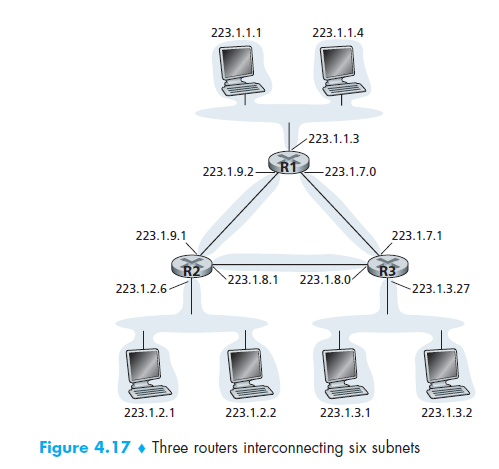
\includegraphics[width=0.7\linewidth, align=c]{images/subnet_example.png}
\end{figure}
\begin{framed}
    \begin{displayquote}
        Core routers in Singapore are running on IPv4. Singtel currently has Singtel has OLT vendors which operate on IPv6, and most of their services are IPv6 ready. They have a tunneling protocol for translating IPv6 internally within the Singtel network to IPv4 to these core routers.
    \end{displayquote}
\end{framed}

\newpage
\subsection{Classless InterDomain Routing (CIDR)}
\begin{itemize}
    \item Address format: \texttt{a.b.c.d/x}
    \begin{itemize}[label=$\circ$]
        \item \textit{x} most significant bits in the address (the prefix) constitute the network portion of the IP address.
        \begin{itemize}[label=\tiny$\blacksquare$]
            \item Organizations usually use a range of addresses with a common prefix.
            \item Hence, when a router outside the organization forwards a datagram whose destination address is inside this organization, they only care about the prefix.
            \item This \textbf{reduces the size of the forwarding table} in the routers, since a single entry of the form \texttt{a.b.c.d/x} will be sufficient to forward packets to any destination within organization.
            \item Sometimes organizations may come together under a subnet for \textbf{route aggregation/ route summarization}.
        \end{itemize}
        \item The remaining ($32-x$) bits are used to distinguish among the devices within the organization.
    \end{itemize}
\end{itemize}
\begin{framed}
    \begin{displayquote}
        Currently there is around 800k prefixes! 60k networks around the world. Singapore comprise of about 1k networks.
    \end{displayquote}
\end{framed}

\subsection{Dynamic Host Configuration Protocol (DHCP)}
DHCP allows host to dynamically obtain its IP address from a network server when it join its network.

\bigskip

\noindent\textbf{How it works - DORA}
\begin{enumerate}
    \item Host broadcast ``DHCP \textbf{D}iscover'' msg [optional]
    \item DHCP server hears the broadcast and responds with ``DHCP \textbf{O}ffer'' msg [optional]
    \item Host requests IP address: ``DHCP \textbf{R}equest'' msg
    \item DHCP server sends address: ``DHCP \textbf{A}ck'' msg
\end{enumerate}

\bigskip

\noindent\textit{Example}
\begin{enumerate}
    \item New connecting host sends a DHCP \textit{request} encapsulated in UDP, IP and Ethernet.
    \item The Ethernet frame \textit{broadcast} on LAN, received at router running DHCP server
    \item Ethernet demuxed to IP demuxed, UDP demuxed to DHCP
    \item DHCP server formulates an ACK containing
    \begin{itemize}[label=$\circ$]
        \item client's IP address
        \item First-hop router for client (if requested)
        \item Name \& IP Address of DNS Server (if requested)
        \item MASK to determine which portion is the network/host (if requested)
    \end{itemize}
    \item Encapsulation of DHCP server, frame forwarded to client, demuxing up to DHCP at client
    \item Client obtains the info inside ACK.
\end{enumerate}

\newpage
\subsection{Network Address Translation (NAT)}
\begin{itemize}
    \item All datagrams leaving local network must have the same single source NAT IP address, but with different src port numbers
    \begin{itemize}[label=$\circ$]
        \item Replace (\texttt{src IP addr, port\#}) of every outgoing datagram to (\texttt{NAT IP addr, new port\#})
        \item Record every (\texttt{src IP addr, port\#}) to (\texttt{NAT IP addr, new port\#}) translation pair in NAT translation table.
    \end{itemize}
    \item Allows local network to use just 1 IP for all devices in the network
    \begin{itemize}[label=$\circ$]
        \item The local network can change address of devices in local network without notifying outside world.
        \item Security: Devices inside local net not explicitly addressable \& visible by outside world.
    \end{itemize}
    \item Allow local network to change ISP without changing addresses of devices in local network
\end{itemize}

\newpage
\section{Lecture 15: Routing Algorithms}
\subsection{Link-state Broadcast Algorithm (LS Algorithm)}
\subsubsection{Properties of the Algorithm}
\begin{itemize}
    \item Centralized: Use global information. Requires each node to first obtain a complete map of the network before running the Dijkstra algorithm.
\end{itemize}

\subsubsection{How it works}
Watch this for explanation of how it the algorithm works: \href{https://www.youtube.com/watch?v=ue-BDS-7Ikw}{\textcolor{blue}{https://www.youtube.com/watch?v=ue-BDS-7Ikw}}. 

\subsubsection{Time Complexity}
\begin{itemize}
    \item Total number of nodes we need to search through over all the iterations is $\displaystyle\frac{n(n+1)}{2}$
    \begin{itemize}[label=$\circ$]
        \item First iteration $n$, 2nd iteration $n-1$ and so on. 
        \item $n + n-1 + ... + 1 = \displaystyle\frac{n(n+1)}{2}$
        \item Hence, \textbf{worst case time complexity} = $O(n^2)$
        \item If we implement the data structure as a heap, can reduce to logarithmic complexity.
    \end{itemize}
\end{itemize}

\subsubsection{Possible Pitfall Scenario - Unequal link costs}
$$c(u,v) \neq c(v,y)$$
For most algorithms, it is assumed that the link costs depend on the traffic carried. And here, the load carried on both directions are not equal.
\begin{figure}[H]
    \centering
    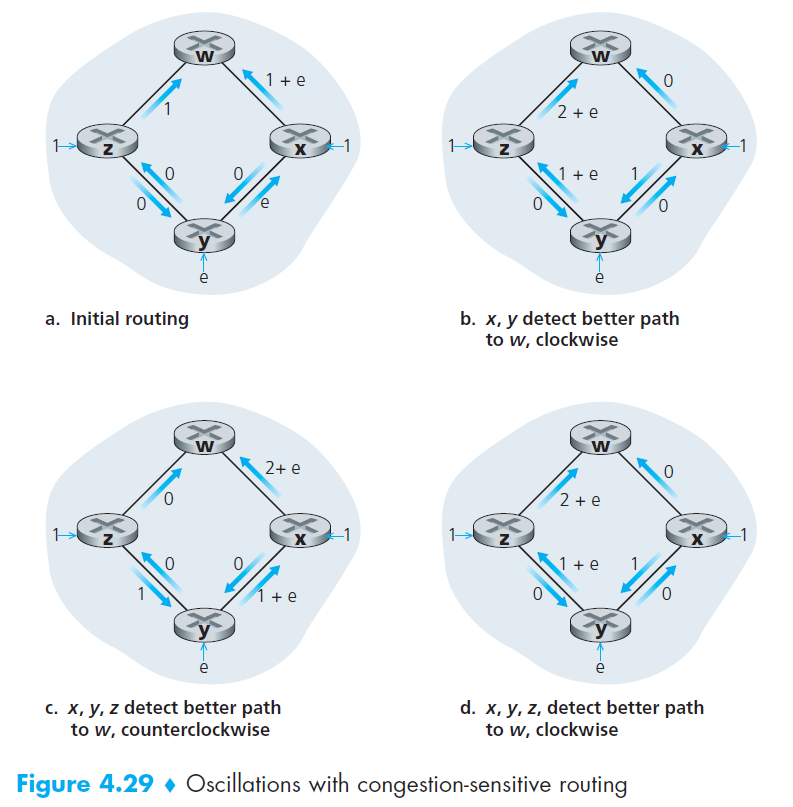
\includegraphics[width=0.65\linewidth, align=c]{images/djikstra_oscillations.png}
\end{figure}

\begin{itemize}
    \item Initialization
    \begin{itemize}[label=$\circ$]
        \item Both $x$ and $z$ originates a unit of traffic destined for $w$,
        \item $y$ injects an amount of traffic equal to $e$, also destined for $w$.
    \end{itemize}
    \item 1st run
    \begin{itemize}[label=$\circ$]
        \item $y$
        \begin{itemize}[label=\tiny$\blacksquare$]
            \item determines that the clockwise path to $w$ has a cost of 1, while the counterclockwise path to $w$ (which it had been using) has a cost of $1 + e$.
            \item So the least-cost path for y is now clockwise.
        \end{itemize}
        \item $x$
        \begin{itemize}
            \item determines that the least-cost path is also clockwise.
        \end{itemize}
    \end{itemize}
    \item 2nd run
    \begin{itemize}[label=$\circ$]
        \item $x$, $y$, and $z$ all detect a zero-cost path to $w$ in the counterclockwise direction, and all route their traffic to the counterclockwise routes.
    \end{itemize}
    \item 3rd run
    \begin{itemize}[label=$\circ$]
        \item $x$, $y$, and $z$ all detect a zero-cost path to $w$ in the clockwise direction, and all route their traffic to the clockwise routes.
    \end{itemize}
\end{itemize}

\medskip

\noindent\textit{Solutions}
\begin{enumerate}
    \item Mandate that link costs do not depend on the amount of traffic carried
    \item Not all routers run the LS algorithm at the same time
    \begin{itemize}[label=$\circ$]
        \item Even though they initially execute the algorithm with the same period but at different instants of time, the algorithm execution instance can eventually become, and remain, synchronized at the routers. To avoid this, randomize the time it sends out a link advertisement.
    \end{itemize}
\end{enumerate}

\subsection{Distance Vector (DV)}
\subsubsection{Properties of the algorithm}
\begin{itemize}
    \item Iterative
    \begin{itemize}[label=$\circ$]
        \item this process continues on until no more information is exchanged between neighbors
        \item requires no signal to ask it to stop
    \end{itemize}
    \item Asynchronous
    \begin{itemize}[label=$\circ$]
        \item does not require all of the nodes to operate in lockstep with each other
    \end{itemize}
    \item Distributed
    \begin{itemize}[label=$\circ$]
        \item each node receives some information from one or more of its directly attached neighbors, performs a calculation, and then distributes the results of its calculation back to its neighbors.
    \end{itemize}
\end{itemize}

\subsubsection{Bellman-Ford equation for Least Cost}
$$ d_{x,y} = \min_v\left[c(x,v) + d_v(y)\right]$$

\newpage
\subsubsection{How it works}
Watch this: \href{https://www.youtube.com/watch?v=x9WIQbaVPzY}{\textcolor{blue}{https://www.youtube.com/watch?v=x9WIQbaVPzY}}
\begin{itemize}
    \item A node $x$ updates its distance-vector estimate when it either sees a cost change in one of its directly attached links or receives a distancevector update from some neighbor.
    \item To update its own forwarding table for a given destination $y$
    \begin{itemize}[label=$\circ$]
        \item what node $x$ really needs to know is not the shortest-path distance to $y$ but instead the neighboring node $v*(y)$ that is the next-hop router along the shortest path to $y$.
    \end{itemize}
\end{itemize}

\subsubsection{Pitfall - Count to infinity problem when a link cost increases}
\textit{Good news travel fast (Lower cost), Bad news travel slow (Higher cost)}

\medskip

\noindent\textit{Solution}
\begin{itemize}
    \item Poisoned Reverse: if $z$ routes through $y$ to get to destination $x$, then $z$ will advertise to $y$ that its distance to $x$ is infinity. $z$ will continue telling this little white lie to $y$ as long as it routes to $x$ via $y$.
    \begin{itemize}[label=$\circ$]
        \item However, does not work for loops involving three or more nodes (rather than simply two immediately neighboring nodes)
    \end{itemize}
\end{itemize}
\newpage
\section{Lecture 16: Scalable Routing}
Routers are usually aggregated into domains known as \textit{autonomous systems} (AS).

\begin{table}[H]
    \centering
    \begin{tabular}{|l|l|}
    \hline
    \multicolumn{1}{|c|}{\textbf{Intra-AS Routing}}                                                                             & \multicolumn{1}{c|}{\textbf{Inter-AS Routing}}                                                                                                                                 \\ \hline
    Gateway has links to other routers in other AS                                                                              & \begin{tabular}[c]{@{}l@{}}Gateway performs inter-domain routing \\ and intra-domain routing\end{tabular}                                                                      \\ \hline
    All routers in AS must run same intra-domain protocol                                                                       & \begin{tabular}[c]{@{}l@{}}Routers in different AS can run different \\ intra-domain routing, but all routers would \\ need to run the same inter-domain protocol\end{tabular} \\ \hline
    Single admin, so no policy decisions needed                                                                                 & \begin{tabular}[c]{@{}l@{}}Admin wants to control over how its traffic\\ is routed, who routes through its net\end{tabular}                                                    \\ \hline
    \begin{tabular}[c]{@{}l@{}}Scalablity less of an issue, can always use \\ hierarchical routing to reduce scale\end{tabular} & Scalability is critical                                                                                                                                                        \\ \hline
    Focus on performance                                                                                                        & Policy may dominate over performance                                                                                                                                           \\ \hline
    \end{tabular}
\end{table}

\subsection{Inter-AS: Border Gateway Protocol (BGP)}
\begin{itemize}
    \item It is a \textbf{path-vector} protocol
    \begin{itemize}[label=$\circ$]
        \item Link cost is not the priority; \textbf{the routing policy is the most important} for BGP Routing.
        \item \texttt{CIDRized Prefix + AS-path + Next-hop}
        \begin{itemize}[label=\tiny$\blacksquare$]
            \item Next-hop: IP addr of gateway router to enter the path (You cannot route AS, only route routers.)
            \item AS-path: Enforce import-policy for paths, avoid looping
        \end{itemize}
    \end{itemize}
    \item Provides each AS a means to
    \begin{itemize}[label=$\circ$]
        \item \textbf{eBGP}: Obtain subnet reachability information from neighbor AS
        \item \textbf{iBGP}: Propagate reachability information to all AS-internal routers
    \end{itemize}
    \item BGP messages are exchanged between peers over semi-permanent TCP connection to advertise paths to different destination network prefixes
    \begin{itemize}[label=$\circ$]
        \item OPEN: \textit{open TCP connection} to remote BGPpeer and authenticate sending BGP peer
        \item UPDATE: Advertises new path / withdraw old path
        \item KEEPALIVE: Keeps connection alive \textit{in absence of UPDATES}. ACKs OPEN request
        \item NOTIFICATION: Report errors in previous msg / Close Connection.
    \end{itemize}
\end{itemize}

\subsubsection{BGP Route Selection}
\begin{itemize}
    \item BGP \textit{sequentially} invokes these rules to select a route
    \begin{enumerate}
        \item  Local Preference value attribute: Policy Decision
        \item Shortest AS-Path
        \item Closest Next-Hop router: Hot Potato Routing
        \item Additional Criteria
    \end{enumerate}
    \item \textbf{Hot Potato Routing}: Choose local gateway that has the \textbf{least intra-domain cost}, without caring about inter-domain cost.
    \item \textit{Habit of Keeping quiet}: If a network X does not want to route from B to C via X, X will not advertise to B a route to C.
\end{itemize}

\subsection{Intra-AS: Interior Gateway Protocols (IGP)}
Routing with Interior Gateway Protocols (IGP).
\begin{itemize}
    \item RIP: Routing Information Protocol
    \item OSPF: \textbf{Open Shortest Path First}
    \begin{itemize}[label=$\circ$]
        \item Area Border: Summarize distances to nets in own area then advertise to other Area Border routers
        \item Backbone: run OSPF routing limited tobackbone
        \item Boundary: Connect to other AS
    \end{itemize}
    \item IGRP: Interior Gateway Routing Protocol
\end{itemize}

\newpage
\section{Lecture 19: Link Layer}
\subsection{Introduction}
\begin{itemize}
    \item \textbf{Main Responsiblity of the Link Layer}
    \begin{itemize}[label=$\circ$]
        \item Transfer datagram from one node to \textit{physically adjacent} node over a link.
        \item Over different links, the datagram is transferred by different link protocols
        \begin{itemize}[label=\tiny$\blacksquare$]
            \item e.g. First Link 802.11, Second Link PPP, ... Last link Ethernet
        \end{itemize}
        \item Each link protocol provide different service.
        \begin{itemize}[label=\tiny$\blacksquare$]
            \item e.g. may or may not provide RDT over link
        \end{itemize}
    \end{itemize}
    \item \textbf{Whether the Link Layer is implemented}
    \begin{itemize}[label=\tiny$\blacksquare$]
        \item Implemented via the combination of hardware, software and firmware in \textit{every host}
        \item Particularly in the \textit{network interface card (NIC)} such as the Ethernet card/802.11 card or a Ethernet chipset. It has a physical interface (physical layer) and a controller (link layer)
        \item Attaches to the host's system buses to connect to the CPU of the host (application, transport, network and link layers), so that it is easier manage the link layer.
    \end{itemize}
\end{itemize}

\subsubsection{Two types of links}
\begin{enumerate}
    \item Point-to-point (PPP)
    \begin{itemize}[label=$\circ$]
        \item Dial-up Access
        \item Link between Ethernet switch and host
    \end{itemize}
    \item Broadcast
    \begin{itemize}[label=$\circ$]
        \item Ethernet
        \item upstream HFC
        \item 802.11 wireless LAN
    \end{itemize}
\end{enumerate}

\subsection{Link Layer Services}
\begin{itemize}
    \item \textbf{Framing, link access}
    \begin{itemize}[label=$\circ$]
        \item Encapsulate datagram into frame, add header and trailer
        \item Channel access if \textit{shared medium} [optional]
        \item "MAC" Address used in frame headers to identify \texttt{src, dest}.
    \end{itemize}
    \item \textbf{Reliable delivery} between adjacent nodes
    \begin{itemize}[label=$\circ$]
        \item Usually used on wireless links that would have \textit{high error rates}. Seldomly used on low bit-error links incude Fiber, Twisted pair, Coaxial Cables.
    \end{itemize}
    \item \textbf{Duplexing}
    \begin{itemize}[label=$\circ$]
        \item Half-duplex: Nodes at both ends of link can transmit \textit{but not at the same time}.
        \begin{itemize}[label=\tiny$\blacksquare$]
            \item There may be collision if the node receive $\geq 2$ signals at the same time, due to simultaneous transmissions (interference).
        \end{itemize}
        \item Duplex: Nodes at both ends of link can transmit at the same time. There will be 1 wire for 1 direction.
        \begin{itemize}[label=\tiny$\blacksquare$]
            \item Utilize Multiple Access Protocol.
        \end{itemize}
    \end{itemize}
\end{itemize}

\newpage
\subsection{Addressing: IP vs MAC}
\begin{table}[H]
    \centering
    \begin{tabular}{|l|l|}
    \hline
    \multicolumn{1}{|c|}{\textbf{IP address}}                                                                              & \multicolumn{1}{c|}{\textbf{MAC address}}                                                                                                                                              \\ \hline
    32-bit                                                                                                                 & 48-bit                                                                                                                                                                                 \\ \hline
    Organizations reserve certain IP address ranges                                                                        & \begin{tabular}[c]{@{}l@{}}MAC address allocation administered by IEEE,\\ manufacturer buys a portion of MAC address space,\\ so first 24 bits configured by manufacturer\end{tabular} \\ \hline
    Dynamically assigned by the network                                                                                    & \begin{tabular}[c]{@{}l@{}}MAC address burned in the NIC ROM.\\ But some are also software configurable.\end{tabular}                                                                  \\ \hline
    \begin{tabular}[c]{@{}l@{}}Uses Decimal Notation\\ e.g. 224.12.13.2/24\end{tabular}                                    & \begin{tabular}[c]{@{}l@{}}Uses Hexadecimal Notation\\ e.g. IA-2F-BB-76-09-AD\end{tabular}                                                                                             \\ \hline
    Network layer forwarding                                                                                               & \begin{tabular}[c]{@{}l@{}}To get frame from one interface to another \\ physically connected interface\end{tabular}                                                                   \\ \hline
    \begin{tabular}[c]{@{}l@{}}Not portable, as address depends on IP subnet\\ to which the node is attached.\end{tabular} & \begin{tabular}[c]{@{}l@{}}Portable, as LAN card containing fixed MAC flat\\ address can be moved from one LAN to another.\end{tabular}                                                \\ \hline
    \end{tabular}
\end{table}

\subsection{Address Resolution Protocol (ARP)}
\textbf{IP address}: Each IP node (host/router) on LAN has a ARP Table that contains IP/MAC address mappings for some LAN nodes, and the TTL time after which address mapping will be forgotten. These ARP tables are created by nodes without intervention from net adminstrator.
\medskip

\noindent So if we know an interface's IP address, we can determine an interface's MAC Address.

\subsubsection{Within the same Local Access Network (LAN)}
\begin{enumerate}
    \item A wants to send datagram to B, but A's ARP table does not have B's MAC Address
    \item A broadcast ARP query packet, containing B's IP Address. All nodes on same LAN will receive this query.
    \item B receives this packet and replies to A with its MAC Address as a frame.
    \item A Caches the IP-to-MAC Address pair in its ARP table until timeout.
\end{enumerate}

\subsubsection{Across LANs}
\begin{enumerate}
    \item All the nodes in the same LAN as A will not know the MAC address of B, who is inside another LAN. But there is a router R between the 2 LANs
    \item A create IP datagram with \texttt{IP src A, dest B}, and put it inside a link-layer frame with \texttt{dest R}. This frame is thus sent from A to R.
    \item R receives this datagram, take it out of the frame and pass it to IP.
    \item R can now create a link-layer frame with \texttt{dest B}, containing the A-to-B IP datagram.
\end{enumerate}

\subsection{Multiple Access Protocol (MAP)}
\begin{itemize}
    \item MAP is a distributed algorithm that determines how nodes share channel (when the node can transmit).
    \item Communication about channel sharing uses the channel itself.
    \item No out-of-band channel for coordinated.
\end{itemize}

\subsection{Ethernet}
The sending adaptor encapsulates IP datagram in an \textbf{Ethernet Frame structure} as such:
\begin{table}[H]
    \centering
    \begin{tabular}{|l|l|l|l|l|l|}
    \hline
    \textbf{Preamble} & \textbf{Destination Address} & \textbf{Source Address} & \textbf{Type} & \textbf{Payload} & \textbf{CRC} \\ \hline
    \end{tabular}
\end{table}
\begin{itemize}
    \item Preamble: 7 bytes with pattern $10101010$ followed by one byte with pattern $10101011$
    \item Address: 6 byte source, destination MAC Address
    \item Type: Indicates higher layer protocol (Mostly IP but others possible, e.g. Novell IPX, AppleTalk)
    \item CRC: Cyclic Redundancy Check at receiver
\end{itemize}

\subsection{Switches}
Switches and Routers are rather similar:
\begin{itemize}
    \item Both are store-and-forward
    \item Both have forwarding tables
\end{itemize}
\begin{table}[H]
    \centering
    \begin{tabular}{|l|l|}
    \hline
    \multicolumn{1}{|c|}{\textbf{Switches}}                                                                   & \multicolumn{1}{c|}{\textbf{Routers}}                                                           \\ \hline
    Link-layer devices                                                                                        & Network-layer devices                                                                           \\ \hline
    \begin{tabular}[c]{@{}l@{}}Learn forwarding table using flooding, \\ learning, MAC addresses\end{tabular} & \begin{tabular}[c]{@{}l@{}}Compute table using routing algorithms, \\ IP addresses\end{tabular} \\ \hline
    \end{tabular}
    \end{table}

\subsubsection{Self-learning}
\begin{itemize}
    \item When the switch receives a frame, it will record sender/location pair in switch table and learn of the location of the sender.
\end{itemize}

\subsection{Virtual Local Area Network (VLANs)}
\begin{itemize}
    \item Made up of switch(es) supporting VLAN capabilities to define multiple virtual LANs over single physical LAN infrastructure
    \item \textbf{Port-based VLANs}
    \begin{enumerate}[label=\roman*.]
        \item \textit{Single physical switch can operate as multiple virtual switches:} Switch ports are grouped by switch management software
        \item \textit{Traffic Isolation:} Frames to/from ports 1-8 can only reach ports 1-8
        \item \textit{Dynamic Membership:} Ports can be dynamically assigned among VLANs
        \item \textit{Trunk port:} Carries frames between VLANs defined over multiple physical switches
    \end{enumerate}
\end{itemize}
802. IQ VLAN frame format
\begin{table}[H]
    \centering
    \begin{tabular}{|l|l|l|l|l|l|l|}
    \hline
    \textbf{Preamble} & \textbf{Destination} & \textbf{Source} & {\color[HTML]{FE0000} \textbf{NEW}} & \textbf{Type} & \textbf{Data (Payload)} & \textbf{CRC} \\ \hline
    \end{tabular}
\end{table}
\noindent\textbf{\textcolor{red}{NEW}}:
\begin{itemize}
    \item 2-byte Tag Protocol Identifier
    \item Tag Control Information
    \begin{itemize}[label=$\circ$]
        \item 3-bit priority field like IP TOS
        \item 1 bit drop eligible indicator
        \item 12 bit VLAN ID field
    \end{itemize}
\end{itemize}
\subsection{Example of all layers together!}
A typical scenario:
\begin{enumerate}
    \item Laptop tries to connect to the Internet and requires the following:
    \begin{enumerate}[label=\roman*.]
        \item its IP address
        \item First-hop router address
        \item DNS server address
    \end{enumerate}
    \item Make a DHCP request encapsulated in IP \& 802.3 Ethernet
    \item Broadcast Ethernet frame on LAN, and the router running the DHCP router receives it.
    \begin{enumerate}[label=\roman*.]
        \item This frame is demuxed to IP, UDP demuxed to DHCP
        \item DHCP Server formulate DHCP ACK containing what the client wants
        \item Encapsulate frame at DHCP server and forward (Switch Learning) through LAN
    \end{enumerate}
    \item Client demultiplexes the DHCP frame and receive the ACK reply
\end{enumerate}

\newpage
\section{Lecture 21: Wireless Networks}
Examples:
\begin{table}[H]
    \centering
    \begin{tabular}{l|l|l|}
    \cline{2-3}
                                                                                                                                                 & \multicolumn{1}{c|}{\textbf{Single hop}}                                                                                                        & \multicolumn{1}{c|}{\textbf{Multiple hop}}                                                                                                                    \\ \hline
    \multicolumn{1}{|l|}{\textbf{Infrastructure}}                                                                                                & \begin{tabular}[c]{@{}l@{}}\textit{WiFi, cellular}\\ Host connect to base station \\ which connects to larger internet\end{tabular} & \begin{tabular}[c]{@{}l@{}}\textit{Mesh Net}\\ Host have to relay through several \\ wireless nodes to connect to larger \\ internet\end{tabular} \\ \hline
    \multicolumn{1}{|l|}{\begin{tabular}[c]{@{}l@{}}No infrastructure\\ (\textbf{No base station + no connection}\\ \textbf{to larger internet})\end{tabular}} & \textit{Bluetooth}                                                                                                         & \textit{MANET, VANET}                                                                                                                    \\ \hline
    \end{tabular}
\end{table}

\subsection{802.11 Wireless LAN}
\begin{itemize}
    \item Basic Service Set (BSS) in infrastructure mode consists of wireless hosts and access point
    \item Host communicates with a base station, known as an access point (AP).
    \item 802.11b spectrum divided into 11 channels at different frequency
    \begin{itemize}[label=$\circ$]
        \item Admin choose frequency for AP
    \end{itemize}
    \item Channel can be same as that chosen by neighboring AP, which may result in \textbf{interference}
    \begin{itemize}[label=$\circ$]
        \item Under \textbf{Carrier Sense Multiple Access} (CSMA)
        \begin{itemize}[label=\tiny$\blacksquare$]
            \item \textit{Collision Detection}: Collisions are detected within short time to reduce channel wastage
            \begin{itemize}[label=\tiny$\blacksquare$]
                \item Easy in wired LANs: can measure signal strength, and compare transmitted, received signals
                \item Difficult in wireless LANs: Received signal strength overwhelmed by local transmission strength
            \end{itemize}
            \item \textit{Collision Avoidance:}
            \begin{itemize}[label=\tiny$\blacksquare$]
                \item Sender Channel sensed idle $\rightarrow$ transmit entire frame
                \item Sender Channel sensed busy $\rightarrow$ defer transmission by starting random \textit{backoff time} and transmit when timer expires. \textit{This interval increases exponentially if no ACK.}
            \end{itemize}
        \end{itemize}
    \end{itemize}
    \item Host associates with an AP by scanning channels, listening for \textbf{beacon frames} containing AP's name (SSID) and MAC address and selecting one to associate with
    \begin{itemize}[label=$\circ$]
        \item There are 2 types of scanning: Passive, Active
        \begin{itemize}[label=\tiny$\blacksquare$]
            \item Passive: APs will send beacon frames
            \item Active: Host broadcast Probe Reuqest Frame + AP will send Probe Response Frames
        \end{itemize}
        \item Then, the host will send Association Request Frame to the selected AP and the selected AP will send Association Response Frame back.
        \item Typically run DHCP to get IP address in the selected AP's subnet
    \end{itemize}
\end{itemize}

\subsubsection{Mobility within same subnet}
\begin{itemize}
    \item When hosts are \textbf{moving between diff APs in the same subnet}, then the self-learning switch will see frame from the host and remember which switch port can be used to reach the hosts.
    \begin{itemize}[label=$\circ$]
        \item If diff subnets, then the host will probably lose connection.
        \item Otherwise, OUT OF SYLLABUS
    \end{itemize}
\end{itemize}

\subsubsection{Rate Adaptation}
Rate adaptation allows transmission to be done at different rates within the wireless network, depending upon the network conditions.
\begin{itemize}
    \item Adaptor can detect channel condition in real-time
    \item Plotted in a Signal Noise Ratio (SNR) vs Bit Error Rate (BER) graph
    \item As the mobile moves away from base station
    \begin{itemize}[label=$\circ$]
        \item BER $\uparrow$, SNR $\downarrow$
        \item When BER becomes too high, switch to a lower transmission rate but with lower BER.
    \end{itemize}
\end{itemize}

\subsubsection{Power Management}
Beacon Frame: Contains list of mobiles with AP-to-mobile frames waiting to be sent
\begin{enumerate}
    \item Node stays awake if AP-to-mobile frames are to be sent.
    \item Otherwise node tells AP ``I am going to zzz until next \textbf{beacon frame}''
    \item AP say ``ok then i don't transmit frames to you''
    \item Node autowakes up before next beacon frame.
\end{enumerate}

\subsection{Mobile Networks}
\subsubsection{Cellular Network Architecture}
\textit{Components of the architecture}

\medskip
\noindent 2G:
\begin{itemize}
    \item BTS: Base Transceiver Station
    \item BSC: Base Station Controller
    \item MSC: Mobile Switching Center
\end{itemize}
\noindent 3G:
\begin{itemize}
    \item SGSN: Serving GPRS Support Node
    \item GGSN: Gateway GPRS Support Node
\end{itemize}
\newpage
\noindent 4G:
\begin{itemize}
    \item UE: User Element
    \item MME: Mobility Management Entity
    \item HSS: Home Subscriber Server
    \item S-GW: Serving Gateway
    \item P-GW: Packet data network Gateway
    \item EPC: Evolved Packet Core
\end{itemize}
\begin{table}[H]
    \centering
    \begin{tabular}{|c|l|l|}
    \hline
    \textbf{Network} & \multicolumn{1}{c|}{\textbf{What changed}}                                                                                                                            & \multicolumn{1}{c|}{\textbf{Components}}                                \\ \hline
    3G               & \begin{tabular}[c]{@{}l@{}}New Cellular Data Network operates in \\ parallel with existing cellular voice network.\\ Voice network is unchanged in core.\end{tabular} & SGSN, GGSN                                                              \\ \hline
    4G               & \begin{tabular}[c]{@{}l@{}}No more separation between voice and data.\\ All traffic is carried over IP core to gateway.\end{tabular}                                  & \begin{tabular}[c]{@{}l@{}}UE, MME, HSS,\\ S-GW, P-GW, EPC\end{tabular} \\ \hline
    \end{tabular}
\end{table}

\subsubsection{Handling Mobility}
\paragraph{Handoff with common MSC}
\begin{enumerate}
    \item Old BSS: ``Oi MSC, i want to HOTO, this is the list of new BSSs''
    \item MSC: ``Ok i set up new path and allocate resources for these new BSS''
    \item New BSS tries to prepare to take over and allocates radio channel for use by mobile
    \item After finishing, the New BSS signals MSC and old BSS ``I am ready''
    \item Old BSS tells new BSS: ``ok now i really HOTO to you''
    \item New BSS signal to activate new channel
    \item Mobile signals via new BSS to MSC: ``Handoff complete''
\end{enumerate}
\medskip
\begin{itemize}[label=\textcolor{OliveGreen}{\Large\checkmark}]
    \item Allows stronger signal to/from new BSS: Continuing connectivity and less battery drain
    \item Load Balancing: Free up channel in current BSS
\end{itemize}

\paragraph{Handoff Between MSCs}\mbox{}

\medskip
\noindent\textit{Distinguishing networks beyond a single MSC}
\begin{enumerate}
    \item Home Network
    \begin{itemize}[label=$\circ$]
        \item Network of cellular provider that a mobile is subscribed to
        \item Network to which the mobile user's permanent phone number belongs
        \item Data Stored in \textbf{Home Location Register} (HLR): The database containing permanent cell phone \#, profile info, info of current location (even outside the home network)
    \end{itemize}
    \newpage
    \item Visited Network
    \begin{itemize}[label=$\circ$]
        \item Network in which mobile currently resides
        \item Data is stored in \textbf{Visitor Location Register} (VLR): Database with entry for each user currently in network.
        \item A visited network can also be home network
    \end{itemize}
\end{enumerate}

\medskip
\noindent\textbf{Multi-MSC Chain}\\
Made up by the Anchor MSC (1st MSC visited during call) + other MSCs that are added onto the end of the chain as the mobile moves to new MSC.
\begin{itemize}
    \item Optional path minimization step to shorten multi-MSC Chain
\end{itemize}

\paragraph{Consequences of mobility}\mbox{}
\begin{itemize}
    \item Performance
    \begin{itemize}[label=$\circ$]
        \item There may be packet loss/delay due to handoff / link-layer retransmissions
        \item TCP may interpret this loss as congestion, and \textit{decrease cwnd unnecessarily}
        \item \textit{Limited bandwidth} of wireless links; wireless behind wired networks by 1-2 orders in terms of speed
    \end{itemize}
    \item Aside from Performance, there should be minimal impact
    \begin{itemize}[label=$\circ$]
        \item Best Effort Service Model remained unchanged.
        \item TCP and UDP can run over wireless mobile
    \end{itemize}
\end{itemize}
\end{document}